\begin{figure}[H]
\centering
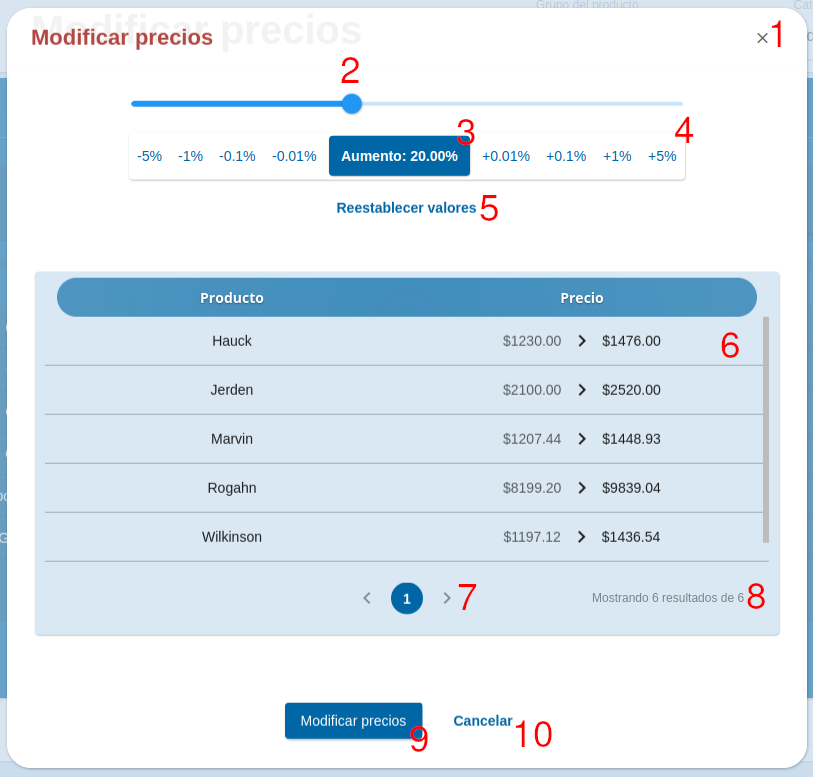
\includegraphics[width=\textwidth,height=\textheight,keepaspectratio]{Escenarios/AD-47-00}
\caption{Escenario - AD-47-00}
\label{fig:AD-47-00}
\end{figure}

Este escenario permite a un usuario modificar los precios de los productos pertenecientes a un determinado grupo de producto, con el botón \textbf{AD-47-01} se podrá cerrar la ventana y volver al escenario \textbf{AD-45-00}.
Si el usuario desplaza el punto sobre la barra deslizable \textbf{AD-47-02} podrá modificar un porcentaje de aumento/descuento que se indica en \textbf{AD-47-03}. Además podrá aumentar o disminuir dicho porcentaje utilizando los botones que se encuentran en \textbf{AD-47-04}. 
Si el usuario hace click en el botón \textbf{AD-47-05} podrá borrar el porcentaje de aumento/descuento que se está indicando. 
En la tabla se podrán encontrar filas como la \textbf{AD-47-06} donde se indica el nombre del producto y precio actual. Si el porcentaje es distinto a 0\% se podrá visualizar el nuevo precio junto con el precio actual. En  \textbf{AD-47-07} se mostrarán las páginas de resultado, pudiendo cambiar de página. En \textbf{AD-47-07} se mostrará cuantos resultados se están visualizando y el total.
Si el usuario hace click en el botón \textbf{AD-47-09} creará el mueble de acuerdo a los campos ingresados y si hace click en el botón \textbf{AD-47-10} cancelará, cerrando la ventana y volviendo al escenario \textbf{AD-48-00}.
\clearpage
